\documentclass[12pt]{article}
%\usepackage[english]{babel}
\usepackage{graphicx}
%\usepackage{framed}
%\usepackage[normalem]{ulem}
\usepackage{indentfirst}
\usepackage{amsmath,amsthm,amssymb,amsfonts}
\usepackage[italicdiff]{physics}
\usepackage[T1]{fontenc}
\usepackage{wrapfig}
\usepackage{lmodern,mathrsfs}
\usepackage[inline,shortlabels]{enumitem}
\setlist{topsep=2pt,itemsep=2pt,parsep=0pt,partopsep=0pt}
\usepackage[dvipsnames]{xcolor}
\usepackage[utf8]{inputenc}
\usepackage[letterpaper, top=0.5in,bottom=0.2in, left=0.5in, right=0.5in, footskip=0.3in, includefoot]{geometry}
\usepackage[most]{tcolorbox}
\usepackage{tikz,tikz-3dplot,tikz-cd,tkz-tab,tkz-euclide,pgf,pgfplots}
\pgfplotsset{compat=newest}
\usepackage{multicol}
\usepackage[bottom,multiple]{footmisc} 
%\usepackage[backend=bibtex,style=numeric]{biblatex}
%\addbibresource{bibliography}
\usepackage{hyperref}
\usepackage[nameinlink]{cleveref} 
\usepackage[titletoc, toc, page]{appendix}


\newtheoremstyle{mystyle}{}{}{}{}{\sffamily\bfseries}{.}{ }{}
\newtheoremstyle{cstyle}{}{}{}{}{\sffamily\bfseries}{.}{ }{\thmnote{#3}}

\theoremstyle{mystyle}{\newtheorem{definition}{Definition}[section]}
%\theoremstyle{mystyle}{\newtheorem{proposition}[definition]{Proposition}}
\theoremstyle{mystyle}{\newtheorem{theorem}[definition]{Theorem}}
%\theoremstyle{mystyle}{\newtheorem{lemma}[definition]{Lemma}}
%\theoremstyle{mystyle}{\newtheorem{corollary}[definition]{Corollary}}
\theoremstyle{mystyle}{\newtheorem*{remark}{Remark}}
%\theoremstyle{mystyle}{\newtheorem*{remarks}{Remarks}}
\theoremstyle{mystyle}{\newtheorem*{example}{Example}}
\theoremstyle{mystyle}{\newtheorem*{examples}{Examples}}
%\theoremstyle{definition}{\newtheorem*{exercise}{Exercise}}
\theoremstyle{cstyle}{\newtheorem*{cthm}{}}


\tcolorboxenvironment{definition}{boxrule=0pt,boxsep=0pt,colback={red!10},left=8pt,right=8pt,enhanced jigsaw, borderline west={2pt}{0pt}{red},sharp corners,before skip=10pt,after skip=10pt,breakable}
%\tcolorboxenvironment{proposition}{boxrule=0pt,boxsep=0pt,colback={Orange!10},left=8pt,right=8pt,enhanced jigsaw, borderline west={2pt}{0pt}{Orange},sharp corners,before skip=10pt,after skip=10pt,breakable}
\tcolorboxenvironment{theorem}{boxrule=0pt,boxsep=0pt,colback={blue!10},left=8pt,right=8pt,enhanced jigsaw, borderline west={2pt}{0pt}{blue},sharp corners,before skip=10pt,after skip=10pt,breakable}
\tcolorboxenvironment{example}{boxrule=0pt,boxsep=0pt,colback={Green!10},left=8pt,right=8pt,enhanced jigsaw, borderline west={2pt}{0pt}{Green},sharp corners,before skip=10pt,after skip=10pt,breakable}
\tcolorboxenvironment{examples}{boxrule=0pt,boxsep=0pt,colback={violet!10},left=8pt,right=8pt,enhanced jigsaw, borderline west={2pt}{0pt}{violet},sharp corners,before skip=10pt,after skip=10pt,breakable}
\tcolorboxenvironment{proof}{boxrule=0pt,boxsep=0pt,blanker,borderline west={2pt}{0pt}{CadetBlue!80!white},left=8pt,right=8pt,sharp corners,before skip=10pt,after skip=10pt,breakable}
\tcolorboxenvironment{remark}{boxrule=0pt,boxsep=0pt,blanker,borderline west={2pt}{0pt}{Cyan},left=8pt,right=8pt,before skip=10pt,after skip=10pt,breakable}
%\tcolorboxenvironment{remarks}{boxrule=0pt,boxsep=0pt,blanker,borderline west={2pt}{0pt}{Green},left=8pt,right=8pt,before skip=10pt,after skip=10pt,breakable}
%\tcolorboxenvironment{example}{boxrule=0pt,boxsep=0pt,blanker,borderline west={2pt}{0pt}{Black},left=8pt,right=8pt,sharp corners,before skip=10pt,after skip=10pt,breakable}
%\tcolorboxenvironment{examples}{boxrule=0pt,boxsep=0pt,blanker,borderline west={2pt}{0pt}{Black},left=8pt,right=8pt,sharp corners,before skip=10pt,after skip=10pt,breakable}
\tcolorboxenvironment{cthm}{boxrule=0pt,boxsep=0pt,colback={gray!10},left=8pt,right=8pt,enhanced jigsaw, borderline west={2pt}{0pt}{gray},sharp corners,before skip=10pt,after skip=10pt,breakable}


\usepackage[explicit]{titlesec}
\titleformat{\section}{\fontsize{24}{30}\sffamily\bfseries}{\thesection}{20pt}{#1}
\titleformat{\subsection}{\fontsize{16}{18}\sffamily\bfseries}{\thesubsection}{12pt}{#1}
\titleformat{\subsubsection}{\fontsize{10}{12}\sffamily\large\bfseries}{\thesubsubsection}{8pt}{#1}

\titlespacing*{\section}{0pt}{5pt}{5pt}
\titlespacing*{\subsection}{0pt}{5pt}{5pt}
\titlespacing*{\subsubsection}{0pt}{5pt}{5pt}

%\newcommand{\sectionbreak}{\clearpage} %Start every section on a new page

%\newcommand{\Disp}{\displaystyle}
%\newcommand{\qe}{\hfill\(\bigtriangledown\)}
%\DeclareMathAlphabet\mathbfcal{OMS}{cmsy}{b}{n}
%\setlength{\parindent}{0.2in}
%\setlength{\parskip}{0pt}
%\setlength{\columnseprule}{0pt}

\title{\huge\sffamily\bfseries GR notes}
\author{\Large\sffamily Yucun Xie}
\date{\sffamily \today}

\begin{document}

\setlength{\abovedisplayskip}{3pt}
\setlength{\belowdisplayskip}{3pt}
\setlength{\abovedisplayshortskip}{0pt}
\setlength{\belowdisplayshortskip}{0pt}
\maketitle

%Custom colors for different environments
\definecolor{contcol1}{HTML}{72E094}
\definecolor{contcol2}{HTML}{24E2D6}
\definecolor{convcol1}{HTML}{C0392B}
\definecolor{convcol2}{HTML}{8E44AD}

\begin{tcolorbox}[title=Contents, fonttitle=\huge\sffamily\bfseries\selectfont,interior style={left color=contcol1!40!white,right color=contcol2!40!white},frame style={left color=contcol1!80!white,right color=contcol2!80!white},coltitle=black,top=2mm,bottom=2mm,left=2mm,right=2mm,drop fuzzy shadow,enhanced,breakable]
  \makeatletter
  \@starttoc{toc}
  \makeatother
\end{tcolorbox}

\vspace*{10mm}

\begin{tcolorbox}[title=Conventions, fonttitle=\large\sffamily\bfseries\selectfont,interior style={left color=convcol1!40!white,right color=convcol2!40!white},frame style={left color=convcol1!80!white,right color=convcol2!80!white},coltitle=black,top=2mm,bottom=2mm,left=2mm,right=2mm,drop fuzzy shadow,enhanced,breakable]
  \begin{enumerate}

    \item Greek index (e.g. $\alpha, \beta, \mu, \nu$) take value from \{0, 1, 2, 3\}.
    %\item Events denoted by cursive capitals  (e.g. $\mathscr{A}, \mathscr{B}, \mathscr{E}$).
    \item $(x^0, x^1, x^2, x^3) \equiv (t, x, y, z) \equiv x^{\alpha}$.
    \item Latin index (e.g.$ i, j, k$) take value from \{1, 2, 3\}.
    \item Natural units ($c=1$).
    \item Einstein summation convention $ds^2 = g_{\mu \nu} x^{\mu} x^{\nu}=
    \sum_{\mu=0}^{3} \sum_{\nu=0}^{3}g_{\mu \nu} x^{\mu} x^{\nu}$.
    \item Metric sign $(-, +, +, +)$.

  \end{enumerate}
\end{tcolorbox}

\newpage

%begin here ---------------------------------------------------------------------------------------------
\section{Differential Geometry}

\subsection{Manifolds}
Mathematically, specetime is a \textbf{manifold}.
\begin{definition}
  An n-dimensional manifold is a set that can be parameterized continuously by n independent real coordinates for each point.
  If a manifold is differentiable at each point, it is a \textbf{differentiable manifold}.
\end{definition}
\begin{definition}
  A coordinate system (also called chart) is n labels uniquely with each point of an n-dimensional manifold through a one-to-one mapping from
  $\mathbb{R}^n$ to $M$.\\
  Generally, more than one charts are required to cover entire manifold, which called \textbf{atlas}.
\end{definition}
\begin{definition}
  Cartesian product $X \times Y$ is set of all possible ordered pairs of element which one from $X$ and one from $Y$.
\end{definition}
Subset of points within a manifold form curves and surfaces. 
Our spacetime is a 4-dimensional \textbf{pseudo-Riemannian manifold}
which is a differentiable manifold with some additional structures.
\begin{remark}
  Manifolds also have a important property which a n-dimensional manifold locally \textbf{homeomorphism} to $\mathbb{R}^n$. See the discussion of
  topology for definition of homeomorphism. Basically this mean a small enough region on manifold is looks same as flat space.
  For example, surface of the Earth is a 2-sphere $S^2$, but look at the ground around you, it seems flat.
\end{remark}

\subsubsection{Maps Between Manifolds}
pullback 
pushforward

\subsection{Tensor}
Tensor is a quantity that have same form in all coordinate system.
Tensor does not have components naturally, but when we choose specific coordinate system, we can write down its components.
Tensor have \textbf{Covariance}, which mean it follow a specific transformation law.

\subsubsection{Vector and Dual Vector}
At each point $P$ of a n-dimensional differentiable manifold, there is a n-dimensional vector space 
which basis is defined by directional derivative at $P$ for curves passing through $P$. 
This vector space is called \textbf{tangent space}. This space contains all \textbf{vectors} at point $P$.
There is also another vector space whose basis is defined by evaluating the gradients of curves passing through $P$ at $P$.
This space is called \textbf{cotangent space}, which contains all \textbf{dual vectors} at point $P$.\\
Vectors and dual vectors are local to a point.\\
Set of all tangent space in a manifold form a \textbf{tangent bundle}, and set of all cotangent space on a manifold
form a \textbf{cotangent bundle}. They are example of \textbf{fiber bundle}.
\begin{definition}
  fiber bundle is a manifold which is locally the cartesian product of base space and fiber space, but not globally.
\end{definition}

\subsubsection{Tensor Notation}
A tensor with \(k\) upper indices and \(l\) lower indices 
\[T^{\mu^1 \mu^2 \mu^3 \cdots \mu^k}_{\nu^1\nu^2\nu^2\cdots \nu^l}\]
is the cartesian product of k vectors and l dual vector. Which map k dual vectors and l vectors to a real number.


\subsubsection{Tensor Transformation Law}
When we changing coordinate system, tensor components transform follow \textbf{tensor transformation law}.
\begin{definition}
  Tensor components in new coordinate system \((\alpha'\beta'\mu'\nu'\cdots)\) can be express as 
  \[T^{\alpha'\beta'\cdots}_{\mu'\nu'\cdots} = 
    \frac{\partial x^{\mu}}{\partial x^{\mu'}}\frac{\partial x^{\nu}}{\partial x^{\nu'}}\frac{\partial x^{\alpha'}}{\partial x^{\alpha}}
  \frac{\partial x^{\beta'}}{\partial x^{\beta}} \cdots
  T^{\alpha\beta\cdots}_{\mu\nu\cdots}\]
\end{definition}
Each upper indice is covariance with coordinate transform, each lower indice is contravariance with cooordiante transform.
If some quantity obey tensor transformation law, it is a tensor. If a tensorial equation is hold in one coordinate system,
it is hold in all coordinate 
system because both side are following same law to transform.

\subsection{Connection}
Connection is an additional structure inposed into manifold. 
There is no naturally defined connection between tangent space at each point on a manifold,
so we can define this additional structure. 
The manifold equip with a flat, torsion-free connection is called \textbf{affine manifold}.
\subsubsection{Covariant Differentiation}

\begin{proof}
  Here is a proof shows that connection not a tensor by show connection does not obey tensor transformation law.
  \begin{align*}
    \begin{split}
      \nabla_{\beta'}e_{\alpha'} & = \Gamma^{\gamma'}_{\alpha'\beta'}e_{\gamma'} \\
      &= \frac{\partial x^{\beta}}{\partial x^{\beta'}}\nabla_{\beta}(\frac{\partial x^{\alpha}}{\partial x^{\alpha'}}e_{\alpha})\\
      &= \frac{\partial x^{\beta}}{\partial x^{\beta'}}(\frac{\partial}{\partial x^{\beta}}\frac{\partial x^{\alpha}}{\partial x^{\alpha'}}e_{\alpha}
      + \frac{\partial x^{\alpha}}{\partial x^{\alpha'}} \Gamma ^{\gamma}_{\alpha\beta} e_{\gamma})\\
      &= \frac{\partial x^{\beta}}{\partial x^{\beta'}}\frac{\partial}{\partial x^{\beta}}\frac{\partial x^{\alpha}}{\partial x^{\alpha'}}e_{\alpha}
      + \frac{\partial x^{\beta}}{\partial x^{\beta'}}\frac{\partial x^{\alpha}}{\partial x^{\alpha'}} \Gamma ^{\gamma}_{\alpha\beta} e_{\gamma}\\
      &= \frac{\partial x^{\beta}}{\partial x^{\beta'}}\frac{\partial}{\partial x^{\beta}}\frac{\partial x^{\alpha}}{\partial x^{\alpha'}}\frac{\partial x^{\gamma'}}{\partial x^{\alpha}}e_{\gamma'}
      + \frac{\partial x^{\beta}}{\partial x^{\beta'}}\frac{\partial x^{\alpha}}{\partial x^{\alpha'}} \frac{\partial x^{\gamma'}}{\partial x^{\gamma}} \Gamma ^{\gamma}_{\alpha\beta}  e_{\gamma'}\\
    \end{split}
  \end{align*}
  \\
  which yield \[\Gamma^{\gamma'}_{\alpha'\beta'} = \frac{\partial x^{\beta}}{\partial x^{\beta'}}\frac{\partial}{\partial x^{\beta}}\frac{\partial x^{\alpha}}{\partial x^{\alpha'}}\frac{\partial x^{\gamma'}}{\partial x^{\alpha}}
    + \frac{\partial x^{\beta}}{\partial x^{\beta'}}\frac{\partial x^{\alpha}}{\partial x^{\alpha'}} \frac{\partial x^{\gamma'}}{\partial x^{\gamma}} \Gamma ^{\gamma}_{\alpha\beta}\]
  There is an extra term in transformation of connection, so connection is not a tensor.
\end{proof}

\subsection{Geodesics}
\subsection{Riemann Tensor}

\section{Gravitation}
\subsection{Equivalence Principle}
\subsection{General Covariance Principle}
\subsection{Einstein's Equation}

\section{Black Holes}
\subsection{Schwarzschild}
\subsection{Kerr}

\section{Gravitational Radiation}
\subsection{Linearized Gravity}
When the gravitational field are weak, the metric take following form :\[g_{\mu\nu} = \eta_{\mu\nu} + h_{\mu\nu} \]
which we treat the gravitational field as a perturbation of flat spacetime metric.
\subsection{Effect of GW on matter}
\section{Cosmology}


\newpage
\appendix
\addcontentsline{toc}{section}{Appendix~}

\section{Special Relativity}


\subsection{Spacetime}
In spacial relativity, we discard the absolute concept of time, in contrast, we add time to our coordinate system, 
now we have a 4-dimensional \textbf{spacetime}.
\begin{definition}
  Inertial coordinate \\
  The coordinate system must satisfy three property to be consider inertial coordinate:
  \begin{enumerate}
    \item The distance between two points are independent of time.
    \item The clocks at every points ticking off time coordinate $t$ at same rate.
    \item The geometry of space is always flat.
  \end{enumerate}
\end{definition}

\begin{figure}[ht]
  \begin{center}
    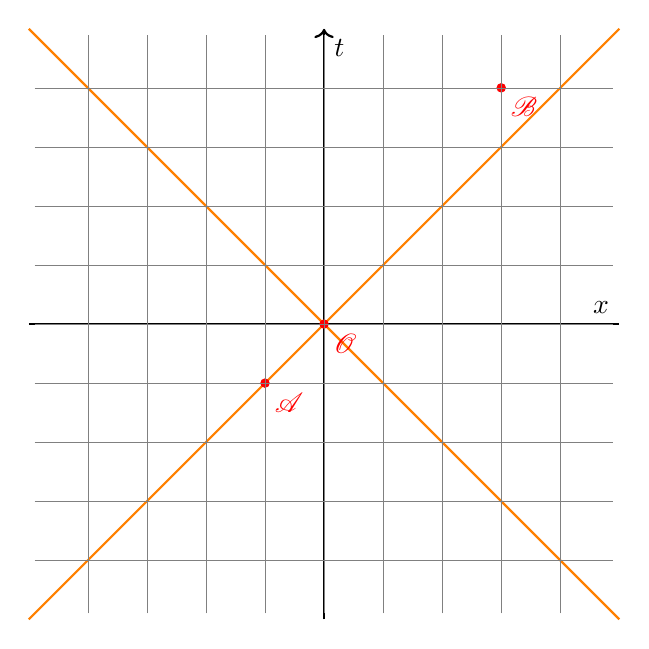
\begin{tikzpicture}[scale = 0.75]
      %\draw[orange, thick] (-5,0) -- (5,0);
      %\draw[orange, thick] (0,-5) -- (0,5);

      \draw[thick,->] (0,-5) -- (0,5) node[anchor=north west] {$t$};
      \draw[orange, thick] (-5,-5) -- (5,5);
      \draw[orange, thick] (-5,5) -- (5,-5);
      \draw[thick] (-5,0) -- (5,0) node[anchor=south east] {$x$};
      \filldraw[red] (-1,-1) circle (2pt) node[anchor=north west] {$\mathscr{A}$};
      \filldraw[red] (0,0) circle (2pt) node[anchor=north west] {$\mathscr{O}$};
      \filldraw[red] (3,4) circle (2pt) node[anchor=north west] {\(\mathscr{B}\)};
      \draw[step=1cm,gray,very thin] (-4.9,-4.9) grid (4.9,4.9);

    \end{tikzpicture}
    \caption[]{two events with coordinate $(-1, -1, 0, 0)$ and $(4, 3, 0, 0)$. Orange line is light's worldline.}
  \end{center}
\end{figure}

The event in 4-D spacetime is defined by a set of coordinate \((t, x, y, z)\).
For simplicity, we assume those events have $y=0, z=0$ so that we can draw a 2D graph to represent them.\\
Analog to Euclidean geometry, just like the euclidean distance \(\Delta l^2 = \Delta x^2 + \Delta y^2 + \Delta z^2\), we define the
\textbf{spacetime interval} $\Delta s^2 = - \Delta t^2 + \Delta x^2 + \Delta y^2 + \Delta z^2$.

\begin{remark}\leavevmode
  There are a lot different conventions to define the sign of interval, here we just use the popular one \((-,+,+,+)\).
\end{remark}
\begin{example}\leavevmode % This is needed to start the list in the next line so it won't be misaligned
  \\Interval for the two events in Figure 1 is $\Delta s^2 = - \Delta t^2 + \Delta x^2 + \Delta y^2 + \Delta z^2 = -9$.
\end{example}
The universality speed of light means that $\frac{\Delta r}{\Delta t} = \frac{\sqrt{\Delta x^2+ \Delta y^2 + \Delta z^2}}{\Delta t}=1$
are always hold, then we can then write the interval
$\Delta s^2 = - \Delta t^2 + \Delta x^2 + \Delta y^2 + \Delta z^2 = 0$. This experimental fact yield all laws of special relativity.
%Due to universal speed of light, interval is invariant change of inertial coordinate, this means that $\Delta s^2 =\Delta \bar{s}^2$ 
%which $\Delta \bar{s}^2$ is $\Delta s^2$ in another inertial coordinate system.\\
\\
When the interval $\Delta s^2$ is less than 0, we call the seperation bewteen events is \textbf{timelike};
When the interval $\Delta s^2$ is equal to 0, we call it \textbf{lightlike} or null;
When the interval $\Delta s^2$ is greater than 0, we call it \textbf{spacelike}.
%The $x^{\mu}=\{x^0,x^1,x^2,x^3\} =\{t, x, y, z\}$ is a set of coordinate.


\subsection{Energy and Momentum}
\subsection{Fluid}

%\section{Skipped proof}

\section{Topological Space}

\section{Lie Algebra}


\section{Property for some tensors}
%Property for tensor used in GR:
\begin{align*}
  \begin{split}
    F_{\mu\nu} &= - F_{\nu\mu}\\
    T_{ij} &= T_{ji}\\
    g_{\mu\nu} &= g_{\nu\mu}\\
    \Gamma ^{\lambda}_{\mu\nu} &= \Gamma^{\lambda}_{\nu\mu} \text{ (Torsion free)}\\
    R_{\alpha\beta\mu\nu} &= -R_{\beta\alpha\mu\nu}\\
    R_{\alpha\beta\mu\nu} &= -R_{\alpha\beta\nu\mu}\\
    R_{\alpha\beta\mu\nu} &= R_{\mu\nu\alpha\beta}\\
    R_{\alpha\beta\mu\nu} + R_{\alpha\nu\beta\mu} + R_{\alpha\mu\nu\beta} &= 0 \\
    R_{\alpha\beta} &= R_{\beta\alpha}
  \end{split}
\end{align*}

\end{document}